\documentclass[letterpaper]{article}
\usepackage{amsmath,amssymb,amsfonts,textcomp}
\usepackage[spanish]{babel}
\usepackage[utf8]{inputenc}
\usepackage[right=2.5cm, left=2.5cm, top=2.5cm, bottom=2.5cm]{geometry}
\usepackage{enumerate}
\usepackage{nicefrac}
\usepackage{setspace}
\usepackage{url}
\usepackage{listings}
\usepackage{graphicx}

\usepackage{graphics}
\usepackage{epsfig}
\usepackage{color}

\onehalfspacing

\title{{\bf Radiosity} \\ \large Computación Gráfica II}
\author{Julio C. Castillo 02--34745 \\ César Romero 02--35409}

\begin{document}

%\allowdisplaybreaks
\maketitle
\begin{abstract}
  Existen varios modelos de iluminación global en computación gráfica
  que buscan crear imágenes reales que no son posibles de generar
  usando el tradicional modelo Phong. Presentamos una implementación
  de Radiosity que permite crear imágenes para distintas escenas sin
  ninguna configuración especial y con parámetros controlados por el
  usuario para controlar la calidad de la imagen generada y visualizar
  detalles que pueden facilitar la comprensión del algoritmo.
\end{abstract}

\section{Introducción}
\label{sec:intro}
% TODO: poner aqui que lo propuso Goral et al. en 1984 y que esta
% basada en los principios de tranferencia de calor entre superficies
% en un ambiente cerrado. Paper original: \cite{goral84}
Radiosity es un algoritmo de iluminación global usado en computación
gráfica cuya finalidad principal es producir imagenes que luzcan
reales calculando el comportamiento de la luz en escenas compuestas
unicamente de superficies difusas.


El objetivo principal de esta implementación es conocer los detalles
del algoritmo, que usualmente no quedan claros con una simple revisión
bibliográfica, y reforzar conocimientos de computación gráfica que
hemos ido adquiriendo recientemente.

Dividimos nuestra implementación en etapas que nos facilitaron la
comprensión e implementación del algoritmo y que explicaremos a
continuación con cierto nivel de detalle.

\section{Representación del Mundo}
Antes de poder hacer el cómputo necesario para crear una imagen de la
escena que queremos reproducir, es necesario tener claro como se
modeló el mundo sobre el cual se realizaron los cálculos. A
continuación explicamos con detalle nuestra representación tanto en el
archivo de entrada (del cual son leídos los datos), como en memoria
(sobre los cuales se realizan los cálculos)

\subsection{El archivo: Formato MDLA}
\label{sec:mdla}
Para la especificación del archivo de entrada se utilizó el formato
MDLA\cite{mdla}. Un formato definido conjuntamente por la Universidad
de Cornell y la Universidad de Indiana. Según los autores, el objetivo
de este formato era crear una forma simple, práctica y rápida de
almacenar modelos de escenas.

Se decidió utilizar este formato principalmente porque ya existe una
especificación de la Caja de Cornell en este formato y fue justamente
esta escena con la que queríamos probar nuestra
implementación. Adicionalmente, está disponible libremente una
librería en C++ que permite leer este tipo de archivos de manera
sencilla.

Es importante destacar que la especificación de la Caja de Cornell
disponible en~\cite{cornellboxdata} define los colores de los
materiales tomando 76 longitudes de onda del espectro visible. En
nuestra implementación las longitudes de onda disponibles en la
especificación original fueron sustituidas por una tripleta RGB que
aproxima al color en cuestión.

\subsection{Estructura en memoria}
\label{sec:struct}
Para representar el ``mundo'' en memoria se utiliza un conjunto de
\texttt{Shape}s. Cada \texttt{Shape} contiene la toda la información
relacionada con una superficie de la escena:
\begin{itemize}
\item Un \texttt{Quad} que contiene la información de los cuatro
  vértices de la superficie.
\item Un vector normal a la superficie.
\item El color o material de la superfice.
\item Una matriz de \textsl{patches} que se generan durante la fase de
  particionamiento.
\end{itemize}

\begin{minipage}[c]{0.6\linewidth}
\begin{lstlisting}[language=C++,frame=single,caption=Representación básica del modelo]

struct Shape{
  Quad vertices;
  Material material;
  Vector normal;
  Quad patches[][];

  void part(float maxarea);
  int parts(float maxares, const Quad& Q);
};

\end{lstlisting}
\end{minipage}

% TODO: poner el codigo del quad

La estructura Quad es la que contiene los puntos que definen al
cuadrilátero y por lo tanto esta se usa para los patches que se crean
durante el particionamiento de la escena y para la definición del
\textsl{Shape} como tal. Esta clase contiene además métodos para el
cálculo del área y centro del cuadrilatero, y para subdividir el
\textsl{Quad} en 4 subregiones iguales. Esto último se utiliza en la
fase de Particionamiento para determinar el número total de patches
que tendrá la escena como se explica en la Sección \ref{sec:part}.

El hecho de tener un método para calcular el área y un vector normal
al plano que conforma cada {\em Quad}, además de un apuntador al
\textsl{Shape} al que pertenece, facilita la implementación del
particionamiento y el cálculo de los \textsl{form-factors} que serán
explicados con mayor detalle en las secciones \ref{sec:part} y
\ref{sec:ff} respectivamente.

\section{Particionamiento}
\label{sec:part}
Inicialmente se pensó en un particionamiento recursivo que fuera
creando patches y los fuera agregando inmediatamente a una lista de
patches, que tendría cada \texttt{Shape}. La idea fue tomada de
\cite{ggems3} que dado un cuadrilátero, lo divide en cuatro secciones
de igual área tal como se observa en la figura~\ref{fig:part}. Esto se
hace promediando las coordenadas de los vértices para obtener el punto
central y simultaneámente ir calculando el punto medio entre cada par
de vértices. Con esta información es posible generar los cuatro nuevos
cuadriláteros. A continuación se muestra el pseudocódigo de este
algoritmo.

\begin{figure}[htbp]
  \centering
  \input{part.pstex_t}
  \caption{Particionamiento de un cuadrilátero en 2D}
  \label{fig:part}
\end{figure}

\begin{lstlisting}[language=pascal,caption=Algoritmo de subdivisión de un cuadrilátero,frame=single,mathescape=True]
procedure splitQuad(q: Quad, var q0,q1,q2,q3: Quad) 
begin
  { calcula el centro y los 4 puntos intermedios entre esquinas }
  center $\leftarrow$  (q[0] + q[1] + q[2] + q[3]) / 4
  mid0 $\leftarrow$ (q[0] + q[1]) / 2
  mid1 $\leftarrow$ (q[1] + q[2]) / 2
  mid2 $\leftarrow$ (q[2] + q[3]) / 2
  mid3 $\leftarrow$ (q[3] + q[0]) / 2

  { construye los 4 nuevos cuadrilateros }
  q0 $\leftarrow$ (q[0], mid0, center, mid3)
  q1 $\leftarrow$ (q[1], mid1, center, mid0)
  q2 $\leftarrow$ (q[2], mid2, center, mid1)
  q3 $\leftarrow$ (q[3], mid3, center, mid2)
end
\end{lstlisting}

La condición de parada sería un área máxima permitida para cada
\texttt{Patch}, es decir, cada \texttt{Patch} es subdividido en cuatro
nuevos \texttt{Patches} hasta que el área de cada uno de los
\texttt{Patches} resultantes es menor que el área máxima
permitida. Esta área es especificada por el usuario con un parámetro
al momento de ejecución. En la Figura \ref{fig:part} podemos ver una
representación de 2 dimensiones de como es esta subdivisión que
mencionamos.

Esta técnica se implementó satisfactoriamente, sin embargo, el orden
en que quedaban almacenados los \texttt{Patches} en memoria
dificultaba el acceso a los vecinos de cada \texttt{Patch} de manera
eficiente. Esto es de particular importancia para la fase de
Renderizado (ver sección \ref{sec:render}) porque para disminuir la
cantidad de artefactos en la imagen final, se usa la información de
los vecinos de cada patch.

Se reimplementó el particionamiento tomando ideas de la técnica
explicada pensando un poco más en el rendering. La subdivisión
recursiva sigue siendo importante porque se usa para determinar un $n$
tal que la cantidad total de \texttt{Patches} en el \texttt{Shape} sea
$n^2$. Los nuevos \texttt{Patches} son ahora creados iterativamente
recorriendo el \texttt{Shape} y almecenados en una matriz de tamaño
$n \times n$ en la clase \texttt{Shape} explicada en la Sección
\ref{sec:struct}. De esta manera podemos en cualquier momento
determinar los \texttt{Patches} vecinos de un vértice cualquiera en
tiempo constante y sin aumentar los requerimientos de memoria.

Una limitación que surge con esta técnica es que todos los
\texttt{Shapes} que definen la escena deben ser rectangulares para que
la escena pueda ser modelada y sintetizada por nustro
algoritmo. Cualquier \texttt{Shape} definido en el archivo de entrada
que no cumpla con esta restricción no dará error, pero será modelado
incorrectamente y mostrará resultados probablemente inesperados en la
imagen.

Definitivamente, una mejora no trivial pero interesante sería
generalizar nuestra técnica de particionamiento para poder aplicar
nuestro algoritmo a escenas con mayor variedad de figuras que incluyan
conos, cilindros, esferas e incluso toroides.

\section{Cómputo de los \textsl{Form-Factor}}
\label{sec:ff}
Para hacer el cómputo de los \textsl{form-factors} se utilizó un
algoritmo escrito por Filippo Tampieri extraído de~\cite{ggems3}. Este
algoritmo está implementado en C y el cálculo que realiza garantiza
ser muy preciso.

Como se explicó en la sección \ref{sec:part}, para cada subregión del
patch, si esta tiene un área menor que un $\Delta A_r$ definido,
entonces se divide el cuadrilátero en 4 subregiones y se computa
recursivamente el \textsl{form-factor} de cada una. Subdividiendo el
patch receptor en areas cada vez más pequeñas $\Delta A_j$ y
utilizando diferentes aproximaciones constantes de la visibilidad $v$
para cada $\Delta A_j$, la función de visibilidad puede ser aproximada
a cualquier grado de precisión \cite{ggems3}. Así, la contribución de
la fuente $s$ al punto $x$ es
$$\Delta B_r(x)=\rho_rB_s\sum_{j=1}^m(V_jF_{dA_r(x)\rightarrow\Delta A_j}),$$
donde $V_j$ es la fracción de $\Delta A_j$ visible desde $x$.

En la implementación de Tampieri \cite{ggems3} esta función de
visibilidad es externa de manera tal que se adapte a la representación
particular del ``mundo''. El siguiente pseudocódigo muestra el
algoritmo recursivo para computar $\Delta B_r$ que será utilizado en
nuestra implementación

%   $\Delta B_r\leftarrow$ComputeContribution(r(x),s,$\epsilon_B$,$\epsilon_A$);
%   ComputeContribution(r(x),s,$\epsilon_B$,$\epsilon_j$)
%    if CanCull(r(x),s)
%     then return 0;
%     else begin
%      $\epsilon_F\leftarrow\epsilon_B/(\rho_rB_s);$
%      return $\rho_rB_s\cdot$ComputeFormFactor(r(x),s,$\epsilon_F$,$\epsilon_A$);
%      end;

\pagebreak{}
\begin{lstlisting}[language=Pascal,frame=single,caption=Cómputo de form-factors,mathescape=True]

  ComputeFormFactor(r(x),s,$\epsilon_F$,$\epsilon_A$)
   begin 
   V$\leftarrow$ComputeVisibilityFactor(r(x),s);
   if V$\leq$0
    then return 0;
   else if V$\geq$1
    then begin
      $F_{dA_r\rightarrow A_s}\leftarrow$ComputeUnoccludedFormFactor(r(x),s);
      return $F_{dA_r\rightarrow A_s}$;
      end;
   else begin
      $F_{dA_r\rightarrow A_s}\leftarrow$ComputeUnoccludedFormFactor(r(x),s);
      if $F_{dA_r\rightarrow A_s}\leq\epsilon_F\;$or$\;A_s\leq\epsilon_A$
        then return $VF_{dA_r\rightarrow A_s}$;
      else begin
        $(s_1,s_2,...,s_m)\leftarrow$SplitPatch(s);
        return $\sum_{j=1}^m$ComputeFormFactor(r(x),$s_j$,$\epsilon_F$,$\epsilon_A$);
        end;
      end;
   end;
\end{lstlisting}

\subsection{Visibilidad}
\label{sec:vis}

En general, en cualquier implementación de este algoritmo, es
importante el cálculo apropiado de la visibilidad entre
\texttt{Patches}. Sin un buen cálculo, no sería posible apreciar
sombras reales e incluso en el \textsl{bleeding} del color entre
objetos de la escena luciría muy poco realista.

Inicialmente la visibilidad se hizo tomando en cuenta los vectores
normales a las superficies que contienen cada uno de los
\texttt{patches} de la escena. El ángulo que se forma entre estos dos
vectores nos permite saber si los patches en consideración ven en la
misma dirección o en direcciones opuestas. Si ven en la misma
dirección puede ocurrir que sean patches vecinos, o que uno le de la
espalda al otro, y en ambos casos esto nos indica que el aporte entre
estos patches debe ser 0. Pero si los patches ven en direcciones
opuestas no podemos realmente determinar si se están viendo porque
para esto es necesario considerar los demás objetos en la escena y
asumir que el aporte entre estos patches es 1 resultaría en una escena
sin sombras y muy poco realista.

En nuestra implementación no sólo nos interesa si un \texttt{Patch} es
visto por otro, sino que también que proporción de este último es
visible. Con esto se determina cuando es necesario ``subdividir'' el
\texttt{patch} que queremos ver para poder hacer un cálculo mas
preciso del \textsl{form-factor}.

Para determinar que proporción del patch $j$ es visible desde el patch
$i$ lanzamos un rayo desde el centro de $i$ en dirección de cada uno
de los vértices de $j$. Si alguno de estos rayos intersecta algún
Shape $S$ de la escena y la distancia desde $i$ a $S$ es menor que la
distancia entre $i$ y el vértice de $j$ hacia donde fue lanzado el
rayo, entonces ese vértice no es visible y nos encontramos en un caso
de oclusión parcial. Si, por el contrario, el rayo lanzado intersecta
directamente al \texttt{Shape} al cual pertenece el patch $j$ decimos
que el vértice es visible y repetimos el cálculo para los vértices de
$j$ restantes.

Para determinar si el rayo lanzado intersecta un Shape $S$ cualquiera
de la escena hacemos varios cálculos de álgebra lineal. Primero
construimos la ecuación del plano $A$ que contiene a $S$ y construimos
la recta $l$ que pasa por el centro de $i$ y por el vértice de $j$ que
queremos verificar si es visible. Con esto podemos hallar el punto $p$
en el que la recta $l$ intersecta a $A$ y poder verificar si el punto
$p$ pertenece realmente a $S$. Para esta última verificación dividimos
el cuadrilátero que forma a $S$ en dos triángulos y sólo nos queda
verificar que $p$ pertenezca a alguno de estos dos
triángulos. $\dagger$ Aquí es necesario poner referencias y quizá
algún dibujo.

Finalmente si sumamos la cantidad de vértices de $j$ que son visibles
desde $i$ y dividimos esta suma entre 4 (la cantidad de vértices de
cualquier patch de nuestra escena), obtenemos la proporción de
vértices del patch $j$ que son visibles desde el patch
$i$. Formalmente, nos interesa el valor de

$$ |\{v:esVisible(i,v) \wedge v \in j\}|\over4$$

donde $esVisible(i,v)$ se sumple sii el vértice $v$ es visible desde
el patch $i$.

Otra manera de realizar el cálculo de la visibilidad es usando OpenGL
directamente. Si a cada \textsl{patch} le asignamos un número unívoco
y este lo interpretamos como un color en la imagen, es posible
determinar que \textsl{patches} son visibles consultando el
\textsl{z-buffer} de OpenGL y cambiando el punto de vista del
observador. Esta técnica es mas eficiente porque implica que buena
parte de los cálculos se hagan directamente sobre la tarjeta gráfica y
por esto consideramos implementarla en un princpio. Por ser mas
compleja, sin embargo, decidimos hacer pruebas iniciales con la
técnica explicada previamente y los resultados fueron satisfactorios
sin que el overhead fuera muy significativo.

\section{Radiosity}
\label{sec:rad}
Para el cómputo de la solución de radiosidad de cada \texttt{patch} de
la escena se utilizó el método de refinamiento progresivo
desrrollado por Cohen \cite{cohen} tal como se describe por Watt \&
Watt \cite{Watt92}. Este método inicia asignando a cada \texttt{patch}
un valor de radiosidad igual a cero o a su valor de
emisividad. Posteriomente se comienza a actualizar las radiocidades de
los patches utilizando el algoritmo que se muestra a continuación.
\pagebreak{}
\begin{lstlisting}[language=pascal,frame=single,mathescape=True]
repeat 
  for each patch $i$
  begin
    Calcular los form-factors de $i$ con el resto de los patches
    for each patch $j \quad (j \neq i)$
    begin
      $\Delta Rad \leftarrow \rho_j \Delta B_i F_{ij}A_i/A_j$
      $\Delta B_j \leftarrow \Delta B_j + \Delta Rad$
      $B_j \leftarrow B_j + \Delta Rad$
    end;   
    $\Delta B_i \leftarrow 0$
  end;
until convergence;
\end{lstlisting}

Cohen llama a esta técnina ``\textsl{shooting}'' puesto que la
contribución del \texttt{patch} $i$ es distribuida a todos los demás
\texttt{patches} de la escena\footnote{La técnica tradicional de
  resolución por medio de Gauss-Seidel se conoce como
  ``\textsl{gathering}'' pues se puede interpretar como si calculara
  la contribucion de todos los \texttt{patches} de la escena al
  \texttt{patch} $i$.}. Esta actualización global, permite ir
dibujando la imagen en cada iteración; la idea es que a medida que se
va avanzando, la calidad y correctitud de la escena va mejorando.

Otro aspecto a considerar del cálculo de radiosidad es que éste debe
realizarce para cada banda de color.  En particular, a mayor número de
bandas de color, mejor resultado se obtiene. Es por esto que la
implementación de la Universidad de Cornell toma en cuenta un total de
76 bandas de colores. Nuestra implementación, sin embargo, hace uso de
sólo 3 bandas de color: rojo, verder y azul.

Los \textsl{form-factors} también dependen de la longitud de onda, sin
embargo, esta consideración se omite para simplificar la
implementación. Por lo tanto, para el cálculo de radiosidad en cada
banda se pueden usar los mismo \textsl{form-factors}.

\section{Renderizado}
\label{sec:render}
La solución de radiosity nos da un valor constante para todo el
\texttt{Patch}. Para minimizar los artefactos en la imagen, sin
embargo, necesitamos los valores para cada vértice de la
superficie. Estos los podemos obtener calculando el promedio de las
radiosidades de las subregiones vecinas \cite{Watt92,cohen85} como se
mencionó también en la Sección \ref{sec:part}.

La solución de radiosity esta constituida números que toman valores
reales. Estos deben ser escalados a un número entre 0 y 255 para poder
introducirlos en OpenGL. Este escalamiento se debe realizar con una
función sigmoidal \cite{tumblin} porque puede haber valores extremos
que son muy similares cuando se muestran en pantalla. Lo que se quiere
es dar mayor relevancia a valores intermedios.

\subsection{Disminución de Artefactos}
\label{sec:smooth}
Al momento de dibujar la imagen tenemos la información de la
radiosidad calculada para cada \texttt{Patch} y en cada
\texttt{Shape}, como se dijo en la Sección \ref{sec:part}, tenemos una
matriz con todos los \texttt{Patches} que le corresponden. Con esta
información podemos disminuir significativamente la cantidad de
artefactos que aparecen en la imagen asignando un color a cada vértice
que va a ser pintado y dejar que OpenGL haga el \textsl{blending}.

Recorremos cada uno de los \texttt{Patches} y cada uno de sus
vértices. Cada vértice tendrá el color que resulte de promediar las
radiosidades de cada uno de los \texttt{Patches} de los que este
vértice forma parte como se muestra en la Figura
\ref{fig:vertex}. Esto lo hacemos en tiempo constante porque tenemos
una matriz de \texttt{Patches} de donde podemos obtener los vecinos de
manera trivial.

\begin{figure}[htbp]
  \centering
  \input{interp.pstex_t}
  \caption{Cálculo de radiosidad en los vértices}
  \label{fig:vertex}
\end{figure}

En los \texttt{Patches} fronterizos (que tienen al menos un lado cuyo
vecino no pertenece al mismo \texttt{Shape}) algunos vértices son
pintados tomando en cuenta sólo uno o dos \texttt{Patches} y no cuatro
como la mayoría. Como se explicó en la Sección \ref{sec:struct} los
\texttt{Patches} están almacenados en el \texttt{Shape} al cual
pertenecen. Esto hace dificil conocer los vecinos \textsl{externos} y
por eso no siempre es posible usar la misma cantidad de información
para calcular el color de cada vértice.

Este problema pudo ser resuelto usando una estructura más complicada
para almacenar los \texttt{Patches} al momento del
Particionamiento. Esto, sin embargo, dificulta la implementación y
disminuye la eficiencia del algoritmo sin producir mejoras muy
significativas en la imagen, en caso de haber alguna. Por esto
decidimos que era mas adecuada la implementación actual y, de hecho,
obtuvimos imagenes considerablemente mejores a medida que aumentaba el
número de \texttt{Patches} en la escena. En la Figura \ref{fig:smooth}
vemos una comparación entre escenas con y sin suavizado. 

\begin{figure}[htbp]
  \centering
  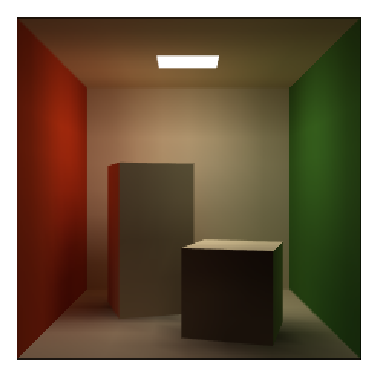
\includegraphics{img/smooth}
  \hspace{2em}
  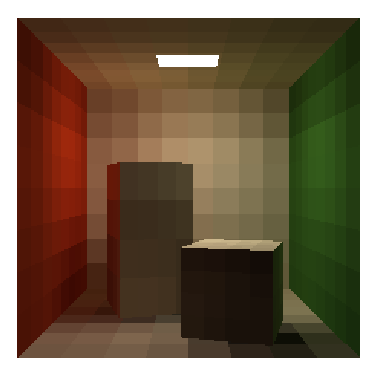
\includegraphics{img/nosmooth}
  \caption{Comparación de dos imágenes de la caja de Cornell generada
    por nuestro algoritmo. A la izquierda con cálculo de radiosidad
    por vértice, a la derecha sin ningún suavizado}
  \label{fig:smooth}
\end{figure}

\subsubsection*{Gamma Correction}

\subsubsection*{Antialiasing}
\label{antialias}
En computación gráfica, aliasing se refiere a la aparición de bordes
``dentados'' o bruscos, pérdida de detalle, aparición de patrones de
moiré, etc. Todos estos fenemenos han sido estudiados \cite{alias1} y
existen técnicas conocidas que ayudan a eliminar o disminuir estos
artefactos.

En nuestra aplicación es necesario aplicar un filtro de antialiasing
para suavizar los bordes y eliminar los bordes ``dentados'' que
aparecen principalmente en la parte superior e inferior de los cubos.

Para realizar el antialias de la imagen final se consideraron dos
técnicas. La primera opción era usar el suavizado de polígonos nativo
de OpenGL \cite[capítulo~6]{redbook}, sin embargo para usar esta
técnica era necesario desactivar el \textsl{z-buffer} y dibujar
primero los polígonos más cercanos al observador y luego los más
alejados. Esta opción se descartó porque en nuetra aplicación esta
restricción no es facil de sastifacer ya que nuestros polígonos están
ordenados para poder acceder rapidamente a sus vecinos, y no para
determinar cuáles están más cerca del punto de visión.

Nuestra segunda opción, y la que finalmente implementamos, es una
técnica que consiste en dibujar varias veces la misma imagen pero
desplazando ligeramente el punto visión \cite{accum} en el eje $x$ y
$y$. Luego se genera la imagen final, que se construye como el
promedio de todas las imagenes desplazadas que se crearon
anteriormente. Para implementar esto de manera eficiente (en hardware,
probablemente), se utiliza el \textsl{accumulation buffer} de OpengGL
\cite{redbook}.

\begin{figure}[htbp]
  \centering
  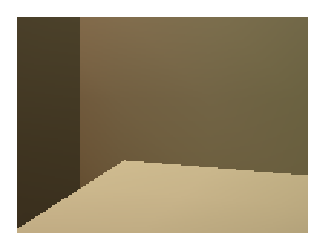
\includegraphics{img/alias}
  \hspace{2em}
  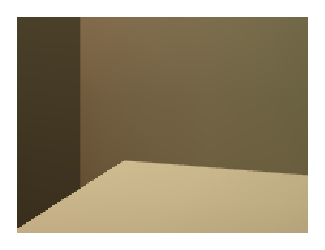
\includegraphics{img/antialias}
  \caption{Comparación de una sección de la caja de Cornell. A la
    izquierda sin antialias, a la derecha con antialias}
\end{figure}

\bibliographystyle{unsrt}
\bibliography{informe}

\end{document}
